\chapitre{Grande bouffe pour Dart Vader, le 26 juillet 2033}{Si on en croit Charles Baudelaire,}{ homme de lettres naguère fort respecté, le mal se ferait sans effort, naturellement, par fatalité et le bien serait toujours le produit d’un art. Pourtant, cette perle de sagesse ne s’applique presque pas dans le cas de Robert Gagnon, maigre vieillard trachéotomisé et édenté surnommé Dart Vader, ce qui fait de l’aphorisme baudelairien un sophisme au lieu d’un truisme. Car pour faire le bien qu’il a choisi de faire, entendre ici «châtier un méchant», le bonhomme a décidé de faire le mal, un mal prémédité et planifié. Quant à la fatalité, si elle a été de la fête, elle ne s’est pas retrouvée à l’origine de ce mal calculé, mais dans son exécution qui s’est brutalement soldée par une conclusion aussi dramatique qu’accidentelle - la vie nous réservant bien des surprises – c’est-à-dire une fin en queue de poisson incarnée dans un plat de crevettes écaillées, cuites et aromatisées à l’ail. }

En début de journée, lorsqu’il a été subir les foudres haineuses de Philippe «Flipper» Dauphin en compagnie de Timothée, son chef de section, Dart Vader a pris bonne note du fait qu’en fin de soirée, on livrerait des plats qu’un traiteur avait préparés pour la réunion du Conseil d’administration du lendemain. Claude Sey, le plus jeune des adjoints de Dauphin, a même précisé l’heure de la livraison, soit entre 21 h 30 et 22 h, moment précis où le concierge vient faire le ménage, ce qui signifie que les portes seront ouvertes. Dans l’esprit de l’ancien noceur de toutes les galères et de tous les tabacs, il ne fait alors aucun doute que le trésor festif sera apporté dans la cuisinette attenante à la salle du Conseil. Dans sa vieille tête malfaisante et rusée, il ne lui reste plus qu’à trouver le moyen de s’approprier une telle merveille. Pas seulement pour faire bombance, mais pour foutre une pagaille monstre dans l’organisation du Flipper. Il fera en sorte que l‘on sache partout que grâce à l’incurie de Dauphin, lui, Robert Gagnon, misérable avaleur de Nutrisuz depuis trois ans, il a pu se livrer à une orgie alimentaire mémorable à même la bouffe de ces salauds du CA.

Le plan qu’il se met dès lors à mijoter sera cousu de fil blanc et d’impondérables, mais il aura le mérite d’être simple. Tant et si bien que Gagnon va l’appliquer à la lettre. Depuis qu’il est pensionnaire au CRG-BSL, il a observé au hasard de ses promenades dans l’établissement – ce qu’on a fini par lui interdire - que la circulation au rez-de-chaussée commençait à se faire rare dans l’heure qui suit la fermeture de la cafétéria et qu’aux alentours de 21 h, il n’y avait plus personne dans les parages, sauf d’éventuels gardiens en Saguewanish. Sauf, également, un préposé à l’entretien qui vient passer l’aspirateur, épousseter ce qui peut l’être, vider les corbeilles et ramasser le pire dans les bureaux et les salles.

C’est ainsi qu’à 21 h, Vader emprunte les escaliers et, reprenant héroïquement son souffle à chaque palier, descend lentement vers le rez-de-chaussée. Il estime qu’en utilisant l’ascenseur, il attirerait davantage l’attention des autorités. Bien sûr, il se sait filmé, mais si on le remarque, ce ne sera que le lendemain quand on soumettra les enregistrements de la soirée et de la nuit à un logiciel de reconnaissance et identification du mouvement (RIM). Ça, c’est le bonhomme Asselin qui le lui avait expliqué l’an dernier.

Rendu en bas, il observe et écoute attentivement. On dirait un rongeur flairant les traces de renard. Convaincu que rien ne bouge ni ne respire, il se glisse furtivement sur sa droite, à la manière d’un ectoplasme, et, les doigts croisés, gagne la toilette des hommes sise de biais, en face de la salle du CA. À l’intérieur, il s’assied dans un cubicule la tête dans les mains et les coudes sur les cuisses. Le bonhomme vient de se placer en mode attente. Mais au préalable, il a accolé sur la porte un écriteau bricolé plus tôt indiquant que cette cuvette était en dérangement. Si jamais quelqu’un entrait, il grimperait sur le siège pour ne pas qu’on lui remarque les jambes; il aurait normalement le temps de le faire puisque les «visiteurs» seraient empêtrés avec leur trottinette. Sauf si c’était le balayeur. Et advenant qu’on veuille quand même pénétrer dans son cubicule, il se ferait dénoncer, ce qui lui vaudrait – il l’acceptait d’avance - un nouveau séjour dans les geôles des Papyblues. Mais, basta ! 

\begin{floatingfigure}[l]{45mm}
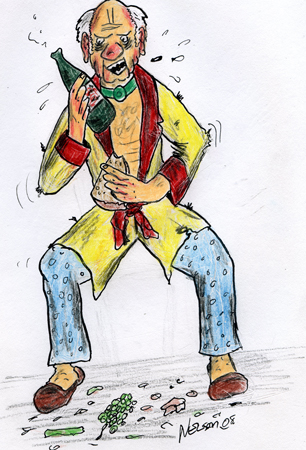
\includegraphics[height=60mm]{corps/chapitre14/img/personnage-vader-bouffe.jpg}
\end{floatingfigure}

Aux cinq minutes à partir de 21 h 30, Dart Vader va écouter à la porte, se risquant même à l’entrouvrir pour tâcher très discrètement d’observer aussi bien le concierge que les livreurs. Il ignorait alors quelle tournure la suite prendrait, mais il misait sur le fait qu’il pourrait peut-être se glisser à l’insu de tous dans la salle du CA et de s’y cacher sous la grande table. Car il y a toujours une grande table, n’est-ce pas ? Faut-il rappeler que son plan était truffé d’impondérables ?

À 21 h 40, un taupin arrive juché sur un chariot électrique et, avec vacarme, arrête son antiquité mal rafistolée devant la porte de la salle suprême. Par la magie de sa boucle d’oreille, il donne le code de la porte laquelle, comme celle des quarante voleurs d’Ali Baba, s’ouvre silencieusement. Sans se douter que des yeux affamés le surveillaient, il y entre avec tout son barda et commence son ménage. Puis, au bout de quinze minutes, il migre dans la cuisinette attenante où il poursuit sa mission hygiénique. C’est à 22 h 07 que deux porteurs de cabarets fermés se pointent en se racontant des trucs du métier qui laissent Dart Vader de glace; par contre, il passe à un poil de défaillir tant leur traînée odoriférante lui apparaît paradisiaque, appétissante, violente, sensuelle, capiteuse, irrésistible. C’est tout juste s’il ne bondit pas leur arracher les contenants.

L’homme de ménage les accueille selon les règles de l’art viril.

- Commençait à être temps, j’suis à veille de tout barrer ! Il me reste rien que le bureau du boss Dauphin à faire !

En déposant sa pile de cabarets, un des livreurs esquisse une excuse.

- Ils se sont aperçus que le céleri faisait pitié. Y ont dû le changer. C’est pour ça qu’on est un peu serré.

- Ouin, ouin !

- Là là, on a encore un voyage de cabarets, p’is on a fini.

- J’en ai pour cinq minutes, répond le concierge en ouvrant la porte séparant la cuisinette du bureau du Flipper, précisément comme elle l’était au moment de l’engueulade du matin.

À ce moment, trois actions se produisent en rafale. Les livreurs se dépêchent vers la sortie, le préposé à l’entretien fait partir son aspirateur chez Dauphin et Dart Vader quitte les toilettes pour se glisser dans la salle du CA. S’il avait encore des doutes sur l’existence d’un Dieu pour les anciens ivrognes et fumeurs extrêmes, ils sont alors annihilés. Car la table du CA est non seulement gigantesque, mais elle dispose sur toute sa longueur, d’une quille de soutien, une médiane en bois foncé qui bloque toute vue ou communication de «dessous de table» entre participants vis-à-vis. Fébrile, le vieillard file se dissimuler à l’autre extrémité du long meuble en acajou, le nez sur la pointe de la quille. Si les livreurs entrent avec leurs contenants, son plan est de se cacher à la droite de l’immense panneau ligneux et si le concierge repasse dans la pièce, il se glissera vers la gauche. Dans les deux cas, l’angle de vision sera obstrué. C’est précisément ce qu’il fait. Les traiteurs reviennent se débarrasser de leur fardeau sans rien remarquer et lancent une vague salutation au préposé qui, à son tour, réapparaît dans la grande salle où, une fois son chariot ramené dans le couloir, il éteint l’éclairage et verrouille la porte.

L’entendant rouler vers les bureaux du fond, le vieux sacripant se relève péniblement en s’appuyant des deux mains sur la table de conférence. Il a réussi ! Il est maintenant enfermé jusqu’au lendemain matin, à moins qu’il ne parvienne à sortir sans se faire attraper. Mais de cela, il doute sérieusement. Un capteur le cafarderait aussitôt qu’il arriverait à ouvrir la porte. Et là, crac ! Au trou ! Bof ! Il a déjà vu pire ! Pour l’instant, le vieillard famélique est seul avec une quarantaine de grands cabarets-contenants pleins de nourriture infiniment troublante. Comme il savait qu’en mettant l’éclairage, il ne faudrait même pas cinq minutes avant qu’un gardien de sécurité ne vienne en vérifier la cause, il s’était alors apporté une halogène à piles, ces torches bonnes pour cinq heures une fois rechargées, qu’il avait «empruntée» au poste de garde du 5e Nord.

Avant de céder à ses envies insupportables, il sort de sa poche intérieure deux feuilles de papier et un tube de colle hydrofuge. À petits pas, il passe dans la cuisinette où il doit se faire violence pour ne pas bondir sur le réfrigérateur, puis il continue dans le burlingue de cette canaille de Flipper. Comme il l’a deviné, ces portes ne sont jamais verrouillées. À l’aide de sa lampe, il colle un des documents écrits à la main, comme au temps des stylos bille, sur le bureau de Dauphin et retourne dans la salle fixer l’autre sur la table du CA, à l’endroit même où siège le président du conseil. Ils devront gratter longtemps avant de pouvoir les enlever. On peut y lire :

    Parce que tu es incroyablement con, Flipper, tu m’as permis de savoir, ce matin quand tu voulais tordre le règlement pour me retourner en prison, qu’il y aurait du vrai manger, ce soir, dans ta cuisinette, à quelle heure on viendrait le porter, le manger, et à quelle heure il n’y aurait plus personne pour m’empêcher de tout le bouffer. Ça fait que je vais bâfrer tout ce que je peux et ce que je ne pourrai pas, mettons que ça arrive, je vais le cochonner pour ne pas en laisser à ta gang de crosseurs du CA. Et comme je te truste pas, que t’es un faux jeton, Flipper, j’ai utilisé le terminal du quanticordi dans le salon communautaire du 5e Nord, pour expliquer à Carl Michaud avec copie conforme à des journalistes et à Thierry-Ian Dennis-Dubeau, le politicien qui aime pas le manger mou, que je crevais de faim dans tes cages à chiens et que pour manger autre chose que de la cochonnerie de Nutrisuz, j’avais dû voler la nourriture du Conseil d’administration. Ce qui fait que tu es en beau joual vert après moi et que je serai sûrement emprisonné à nouveau. À l’heure où tu lis cette feuille, les Papyblues sont probablement déjà en train de se limer les dents. J’ai horodaté le message pour qu’il parte une heure avant que tu entres dans ton bureau. Bye-bye et bonne journée mon cave !

Et comme un prêtre à qui on a interdit de célébrer la messe pendant trop longtemps, le père Gagnon s’approche du réfrigérateur, vaste tabernacle où on a entreposé la manne céleste, et, salivant comme un danois affamé devant un étal de boucher, il transporte tous les récipients dans la grande salle, les plaçant sur l’autel qu’était devenue la table du Conseil. Ensuite, méticuleusement, il les ouvre un à un, jetant les couvercles à bout de bras. Il découvre ainsi une véritable corne d’abondance faite d’amuse-gueules (olives, choux-fleurs, céleris, concombres libanais, cerises de terre, tomates en grappe et biscottes tartinées de foie gras) avec leurs contenants de sauce trois fromages, de la salade choux - carottes râpés au raisins secs, du taboulé, du jambon melon, du saumon mayonnaise, un monceau de petites crevettes de Matane avec un plat de sauce chili, de la confiture d’oignons à l’ancienne, un plateau complet de fromages (morceaux de cheddar blanc et orangé montés en cubes sur mini brochettes, bleu aux relents affolants, gouda en boulettes de cire rouge, emmenthal bien croûté et camembert bas de gamme), un cabaret gorgé de caramboles en tranches, de noix, de raisins verts, de figues et de poires naines, enfin un dernier plat où sont cordés des carrés de gâteaux secs, des tartelettes à l’érable et au coulis de fraise, ainsi que des biscuits à l’amande. Sur le comptoir à côté du frigo, il a remarqué un sac gonflé de petits pains et six bouteilles de Châteauneuf-du-pape, un cru de 2024, dont il a vivement dévissé tous les bouchons et les a ajoutées au désordre gastronomique de la table.

Dans une de ses poches de robe de chambre, il trouve un petit lecteur musical, le truc bête à dix sous où, l’an dernier, il s’était amusé à se télécharger tout sa musique. Il se l’ajuste aux oreilles et, du bout du doigt, navigue jusqu’à Jean-Pierre Ferland. Clic, c’est fait. La fougue du vieux barde lui emplit les émotions.

    Avant de m’assagir
    Avant de jeter l’ancre
    De ménager mon cœur
    De couver ma santé
    Avant de raconter
    Mes souvenirs à l’encre
    De vouloir sans pouvoir
    De compter mes lauriers
    Avant cette saison
    Avant cette retraite
    Je veux sauter les ponts
    Les murs et les hauts bords
    Je veux briser les rangs
    Les cadres et les fenêtres
    Je veux mourir ma vie
    Et non vivre ma mort

Alors, calmement, comme un amant qui se retient d’exulter trop tôt dans une prestation prometteuse, il s’assied, sourit d’aise et entonne le premier chant de sa grande messe. Il s’agit de crudités, dont des tiges de céleri et des pommettes de chou-fleur, ces légumes qu’il engloutissait de façon compulsive quand il était gamin, avant qu’il ne devienne l’ivrogne impénitent qu’il fut envers et contre tous. Sa prothèse dentaire enfilée, il pose, fou de désir, ce geste lourdement codé dans son ADN, geste d’un réconfort sans bornes et qu’il n’a pu oublier en trois ans de manger mou, consistant à se placer un bâton de céleri entre les dents, d’en suçoter le jus, de le croquer bruyamment, de le mastiquer avec délectation et de l’avaler.

    Je veux vivre en mon temps
    Saboter les coutumes
    Piller les conventions
    Sabrer les règlements
    Avant ce coup de vieux
    Avant ce mauvais rhume
    Qui tuera mes envies
    Et mes trente-deux dents
    Et si je le pouvais
    Je ferais mieux encore
    Je me dédoublerais
    Pour vivre comme il faut
    Le jour pour ce qu’il est
    La vie pour ce qu’elle vaut
    Ça c’est mourir sa vie
    Et non vivre sa mort

Malgré l’orgasme, malgré Ferland, il est étonné de la sensation déplaisante qu’il ressent aux gencives. Pour la première fois en trois ans, ses dents artificielles viennent de forcer, de travailler. Aucunement inquiet, Dart Vader poursuit sa marche vers le paradis avec un morceau de chou-fleur. Même désagrément sous les dentiers, additionné cette fois d’un début de tiraillement dans les masséters, ces muscles masticatoires atrophiés pour cause de non-usage. Dans le plat, tout à côté, que lui présente son halogène, il remarque une quantité folle de noix, une des grandes passions de sa terrible vie. Il a tôt fait de s’en mettre une poignée sous la dent. Mais dès qu’il commence à les broyer, la douleur lui devient insoutenable et il doit tout recracher. Inquiet, quelque peu frustré, il plonge la main dans le cabaret de jambon melon et, cette fois, il ne ressent presque pas de pression aux gencives et c’est à peine si ses muscles lui font sentir leur état de déchéance. Pour qu’il en soit autrement, il va devoir y aller à deux mains et se fouler la cavité buccale comme s’il s’agissait d’un moulin à viande. Mais sa fatigue masticatoire devient telle qu’il se fixe au bec le goulot d’un Châteauneuf et qu’il se sert du précieux liquide pour avaler ce qu’il n’a plus la force de mâcher.

- ‘Stie qui est bon, c’te rouge-là !

Et voilà le père Gagnon en train d’écluser pour la première fois en trois ans, un de ces nectars qui, en synergie avec bien d’autres, lui ont fait perdre, tout au long de sa trépidante vie, femmes, emplois et possessions matérielles. Le vieil homme tente ensuite quelques exercices en s’étirant les maxillaires. Puis, le gosier à nouveau empli de rouge papabile, il s’empare d’une pièce de saumon. Il essaie de ne pas trop l’écraser de son râtelier, mais une douleur du fond de la bouche, là où commence l’œsophage, lui témoigne d’une certaine intolérance envers tout ce qui est plus structuré que le Nutrisuz. Prenant une pause de quelques secondes, il repère le taboulé. Une forte pulsion l’entraîne alors à s’y plonger la tête comme un clébard abandonné, une manœuvre déplorable qui lui fait frôler l’étouffement. D’un geste brusque, il propulse le met fautif sur le tapis et, au passage, attrape les fromages. Il taponne d’abord le bleu et, le jugeant assez mou, s’en emplit la trappe à malice. Quelle extase ! Quels souvenirs ! À nouveau, une sérieuse rasade de vin et, derechef, une généreuse poignée de bleu. Comme dans le bon vieux temps ! Éventrant le sac de petits pains «sour dough» de style San Francisco, il en défait un en trois et, comme pour communier, s’en place un morceau dans la bouche.

- Bleu blanc rouge, grince-t-il de sa canule.

Après une pause pipi dont il confie le cadre au bureau de Philippe Dauphin, il continue son festin cette fois avec les biscottes qu’il se contente de lécher pour n’absorber que le foie gras. Et comme il sent que le conduit stomacal va lui exploser, il vide presque le quart de sa bouteille et entreprend de malaxer le tout avec force bruits de succion et de déglutition. C’est à ce moment qu’il aperçoit le plat de crevettes, un des rares mets pour lesquels il aurait tué du temps où il ne s’appelait pas Dart Vader. Il a tôt fait de se purger la bouche sur le siège voisin et d’y engouffrer une solide poignée de crustacés sans même les plonger dans la sauce rouge. Les misérables crevettes ont tellement été cuites et trafiquées qu’il n’est nul besoin de les mastiquer. Il suffit de les arroser de Châteauneuf.

- ‘Stie que c’est bon !

Mais au moment où il s’apprête à s’offrir un troisième service des deux mains, d’étranges sensations commencent à attirer son attention. Des sensations de lourdeur en progression, de picotement croissant dans les extrémités, d’étau en train de se resserrer sur ses côtes, sur ses poumons et sur son cœur, d’air qui ne parvient plus à passer. Presque en panique, le bonhomme s’empare d’une petite brochette de cheddar, se débarrasse vivement du fromage et introduit le bâtonnet dans sa canule qu’il croit obstruée. Du sang gicle alors de la trachée.

Son dernier geste avant qu’il ne s’écrase sur les cadavres de biscottes léchées, sera de s’arracher la canule.

Mais tout cela, Timothée ne le saura qu’au matin et, surtout, quelques jours plus tard quand le docteur Prévost aura pu terminer son travail.

Pour l’instant, il vient de quitter Shimoune qui doit reprendre son boulot et s’en retourne au 5e avec une nouvelle certitude en tête. Il se passe quelque chose de répréhensible au Bic, quelque chose d’explosif et de mortel pour une carrière de politicien, et sa mère, la Maririou, connaît probablement la fine fleur impliquée dans cette histoire. Elle a travaillé à la première élection du Gros Turcotte, d’où la lettre de cette enflure accrochée sur un mur du sous-sol de la rue Crouet. S’il est vrai que les géniteurs Turcotte ne sont pas morts, pourquoi, eux, vivent-ils dans un paradis sous l’aile d’un ministre omnipuissant, alors que son père et sa mère à lui, Timothée-Milet Tardif, croupissent dans la misère noire sur le bras de leur nono de fils ? Tout autre que lui imaginerait dès lors un plan visant à prendre ces accaparateurs la main dans le sac afin d’en tirer des bénéfices pour ses propres parents; car, il y a sûrement quelque chose à faire. Le problème, c’est qu’au moment où Dieu a distribué le talent de stratège aux humains, le pauvre garçon était malheureusement dehors en train de réparer la crevaison que des voyous venaient de lui infliger.

C’est madame Loubert qui le tire de sa réflexion.

- Ronnie Ross dit qu’il n’y a pas d’autres sacs et que va falloir que je m’habitue aux nouveaux.

Ça n’a aucun bon sens !

- Vous dites que les nouveaux coulent ?

- Oui et ils me salissent toute !

Aucun, mais aucun bon sens !

- Venez avec moi, madame Loubert.

Dans son bureau, il tape sur la fonction téléphonique de son terminal et demande les Approvisionnements.

- Direction des Approvisionnements ! fait une voix ménopausée.

- Timothée Tardif, 5e Nord.

- C’est à quel sujet ?

- Au sujet de votre dernière batch de sac à colostomie, ils coulent.

- Un instant, je vous communique avec un agent de procuration.

Quinze secondes de silence suivent où madame Loubert n’ose même pas parler.

- Adrien Dumont, comment puis-je vous aider ?

- Timothée Tardif, 5e Nord.

- Ah, le Motté ! Qu’est-ce qui se passe ?

- Il y a des problèmes avec votre dernière batch de sacs à colostomie, elle est de mauvaise qualité et les sacs tendent à couler.

- P’is ?

- B’en p’is ? Ça fait du dégât et j’ai une patiente qui se plaint.

- Va falloir qu’al endure, on n’en a pas d’autres !

Deux petits fils se touchent alors dans le crâne du CS-1.

- Comment « qu’al endure » ! C’est pas une réponse, ça !

- B’en c’est celle que j’te donne, le Motté !

- Écoute-moi bien, câlisse, si d’ici demain je n’ai pas reçu ici, au 5e Nord, une caisse de sacs de la même qualité qu’avant, je ramasse les pleins de marde qui coulent et je descends te les vider sur ton bureau ! As-tu compris ?

Debout dans le cadre de porte, Ross voit son chef hurler pour la première fois.

- Demain au plus tard, vocifère ce dernier par-dessus les protestations d’Adrien Dumont.

Et il raccroche.

- Motté, Motté, wouo, du calme !

Le CS-1 regarde le préposé.

- J’le connais, moi, Dumont. Si tu cries après, Motté, t’auras jamais rien. Laisse-moi faire, je vais descendre te négocier quelque chose.

- J’m’en câlisse de ce que tu vas faire, Ronnie ! J’exige seulement qu’il me monte une caisse de sacs normaux.

- J’te dis que j’m’en occupe. Tu vas l’avoir ta caisse.

Timothée qui se doute bien de la motivation profonde de Ronnie Ross, n’a aucun doute que madame Loubert pourra compter, demain au plus tard, sur des sacs de qualité. Il sait que Ross est en gamique avec quelques salauds du Centre, dont Adrien Dumont, et il a la conviction, sans les preuves, que son employé a trempé de façon profitable pour sa poche, dans cette livraison de sacs défectueux. Son intérêt est d’empêcher à tout prix qu’un CS-1 quelconque s’énerve, fasse des vagues et agite la fourmilière, ce qui pourra n’être que défavorable à ses affaires.

- Timothée Tardif, bougonne-t-il à son terminal qui vient de lui transmettre un appel.

C’est Claude Sey qui lui apprend avoir été suspendu sans solde, immédiatement après une visite d’Amédée Chicot chez Philippe Dauphin.

- Mon congédiement est désormais une formalité.

- Euh …

- Vous êtes probablement le prochain, monsieur Tardif. Pensez au docteur Bellavance.

Il a raccroché. Qu’est ce que c’est que cette histoire avec le sinistre chercheur du sous-sol ? Le personnage est un peu abject, non ? Car utiliser des corps cliniquement morts pour produire des hormones est une pratique affreuse très discutable. En quoi est-ce que ça pourrait le concerner, lui ce chef de section abusé, ce fils accablé, ce Casanova dérouté, ce binoclard grassouillet dont les cheveux tombent comme des samares à l’automne ? Y a-t-il un rapport entre cette étrange recommandation de Sey et l’affabilité dont l’inquiétant médecin fait habituellement preuve à son endroit ? Pas plus tard qu’hier, il l’a invité à venir visiter sa «petite installation» du sous-sol, celle qui est voisine de l’antre des Papyblues. «On parlera», a-t-il dit.

- J’adore ta madame Bellow, fait la voix de Robespierre derrière lui.

Timothée regarde sa montre.

- Il est 16 h 15; il arrive quoi pour ta copine Béatrice Martin ?

- Elle nous attend chez elle vers 19 h 30. Mais, oh, ce n’est pas ma copine, c’est une amie. Quelqu’un de très bien que tu vas avoir intérêt à connaître.
Comment faire pour être chez Béatrice à 19 h 30, obtenir d’elle ce dont il a besoin pour neutraliser le docteur Gagnon, demeurer poli, tout en étant, une demi-heure plus tard, chez Marie-Odile à l’autre bout de la ville ? La matrone a en effet précisé qu’il devait se pointer à 20 h. Va donc falloir qu’il lui téléphone pour se dégager une plage temporelle suffisante. Quand on sait qu’il y a une semaine à peine, Timothée n’avait jamais pu s’approcher du charme féminin, il y a de quoi s’étonner de le voir maintenant en situation de négocier avec l’une pour pouvoir aller chez l’autre.

- Faut vraiment que j’y sois ?

- Qu’est-ce t’en penses, idiot ? Je passe te prendre chez toi à 19 h. Et, sans te mettre sur ton trente-six, enlève au moins ton uniforme de garde vieux.

En route vers l’ascenseur du personnel, le chef de section songe que son ami a parfaitement raison. Il devrait faire des efforts vestimentaires, au moins quand il se présente chez les gens, surtout lorsqu’il s’agit d’une dame qui vit seule, une très belle femme toute mignonne qui dégage tellement de douceur, d’empathie, de chaleur et de bonté, qu’on en tombe instantanément amoureux. Évidemment, il y a la fatalité, celle qui oblige le rêveur à quitter impérativement son monde onirique pour se concentrer sur la vraie vie, sur ce à quoi il a eu droit, sur son lot, sur cette forte femme qu’il redoute de plus en plus, sur cette femme-flic que l’on surnomme ici la Bitch à Tremblay, sur cette mégère qui lui a ordonné de venir se rapporter à 20 h.

Deux vieux, main dans la main, le saluent.

- Je voulais te remercier pour la petite chambre, chef. T’as pris pour moi contre eux autres. T’es quelqu’un de bien !

- Je n’ai fait que mon travail, monsieur Martel.

L’homme hoche de la tête d’un air entendu et poursuit son chemin. Robespierre est impressionné.

- C’est bien qu’on te dise des choses comme ça, non ?

Mais Timothée ne répond pas. Car, au sortir de l’escalier, dans le no man’s land séparant son service du 5e Centre, Luce Morency vient d’apparaître.

- Et merde !

- C’est la madame du 6e …

- Oui. Va me chercher une couverture, veux-tu Robespierre ? Et envoie un code Magenta au 6e Nord.

Comme si tout était normal, le CS-1 s’approche en souriant de la démente.

- Comment allez-vous, madame Morency ?

La vieillarde le regarde longuement, la mine profondément angoissée, l’air totalement perdu.

- On se connaît ?

Il la prend par la main et la ramène dans la cage d’escalier où il s’assied sur une marche après lui en avoir fait faire autant.

Dans la seconde qui suit, Robespierre réapparaît.

- J’ai envoyé le code Magenta, mais je trouve pas de couverture.

Son ami hausse les épaules et, calmement, sur le ton de la confidence, amorce un énième monologue avec à la vieille dame.

\begin{floatingfigure}[l]{30mm}
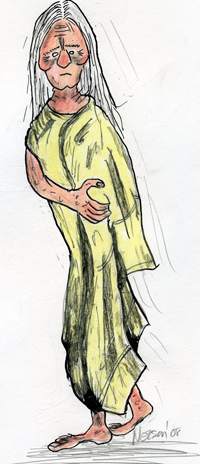
\includegraphics[height=60mm]{corps/chapitre14/img/personnage-morency.jpg}
\end{floatingfigure}

- Vous rappelez-vous au Lac Saint-Mathieu, madame Morency, cet été où il y avait eu une petite fille appelée Julie ? Une petite fille que vous aviez présentée à ma mère comme étant votre nièce de Montréal ? Une petite fille maltraitée que vous aviez accepté de garder pour l’été ? Elle était toute menue, presque maigre. Ses yeux était immenses, bleus comme le ciel quand il fait doux, le printemps. Ses cheveux étaient longs, raides et dorés comme de la corde de chanvre. Et son visage, son visage, je ne me souviens plus de son visage. Ma mère lui avait montré à jouer de l’harmonica, à déchiffrer des partitions.

- Julie …

- Oui, Julie. Elle était tout le temps avec ma mère. Tout le temps. Et elle ne me parlait jamais. Ça me chagrinait un peu parce que j’en étais amoureux, amoureux fou comme en sont capables les petits garçons. Je me cachais sous la roulotte pour la regarder pratiquer sa musique à bouche sur la petite galerie. Je pense qu’elle le savait, mais elle ne faisait voir de rien. Au fil des jours, nous nous étions développé une complicité tacite où j’étais devenu, je pense, un voyeur dissimulé dans la noirceur et elle, une belle que l’on observe furtivement.

- Julie …

- Quand nos vacances se sont terminées, elle a continué de venir chez nous, à Saint-Anaclet. Des fois, madame Morency, vous nous l’ameniez un lundi matin et vous passiez la reprendre le vendredi soir. Pour mon plus grand malheur. Un jour, vous n’êtes plus revenues et je n’ai jamais su ce qu’elle était devenue. J’ai longtemps pensé à elle en rêvant qu’elle arriverait chez nous, qu’elle me tendrait ses bras, qu’elle me dirait vouloir être mon amie. Puis, un jour, je me suis fait à l’idée qu’elle ne reviendrait jamais. Vous vous rappelez de Julie, madame Morency ?

- OK Motté, on la ramène, fait Alain Santerre, un préposé du 6e Nord qui se présente avec une couverture blanche. Merci de t’en être occupé.

Julie, un de ses plus beaux souvenirs d’enfance. Julie dont il n’a jamais su le nom de famille. Morency ? Julie Morency ? Non, cette combinaison ne fonctionne pas. Qu’a-t-elle fait de sa vie ? S’en est-elle sortie ? Elle aurait aujourd’hui 43 ans. Peut-être se souvient-elle de lui. De leur complicité ? Peut-être que s’il la recherchait et la découvrait, qu’elle lui tendrait les bras et qu’elle lui dirait vouloir être son amie ?

Cinq minutes plus tard, les deux compères roulent vers Nazareth. Avec le dispositif personnel polyvalent, alias la boucle d’oreill, de Robespierre, Timothée rejoint Marie-Odile-la-dévorante et lui explique avec douze paires de gants blancs qu’il ne pourra être chez elle à 20 h en raison de sa démarche auprès de cette Béatrice Martin, amie de Robespierre prête à témoigner dans le bon sens de cette histoire épouvantable. La femme-flic trouve la nouvelle plutôt fâcheuse, mais elle dit comprendre la situation. C’est le prix à payer, n’est-ce pas, si on veut se sortir d’un engrenage qui ne peut que nous broyer. Ceci étant dit, en experte de ce genre d’intervention, elle estime qu’il aura besoin d’une heure tout au plus et, en ajoutant trente minutes de voyagement, qu’il pourra être chez elle à 21 h, ce qui est quand même acceptable. Mais à supposer qu’il faille plus de temps, qu’il faille tout expliquer, persuader, négocier, il faudrait prévoir un filet, non ? Pourquoi ne pas s’enlever du stress et s’entendre, disons, pour 22 h ? Ce n’est pas si tard, 22 h !

- B’en on avait dit 20 h, p’is là c’est rendu à 21 h et tu veux qu’on mette ça à 22, gronde Marie-Odile. Tant qu’à y être, pourquoi pas à demain matin ? Écoute donc, es-tu sûr que c’est pour son témoignage que tu vas voir c’te femme-là ? Ne non ! 21 h, c’est une bonne heure; tu vas avoir le temps de tout faire ce que tu as à faire.

- Euh …

- Je t’attends. Travaille bien ! À tantôt mon gros loup !

«Mon gros loup» ? Dieu du ciel ! Il se sent plutôt chèvre accrochée à un piquet, lièvre dans un habitat de martre, gnou en train de courser contre une femelle guépard, carpe dodue dans un bassin à piranhas, voire hamster se sentant observé par une grosse couleuvre. Le couvre-feu est à 21 h, qu’elle a décrété, la maîtresse femme! Cela parce qu’elle entend se faire sauter à 21 h 05 ! Ce qui signifie que lui, il devra être en mode service-service dès 21 h 04. Le mode d’emploi est très simple, chère madame. Vous appuyez ici, c’est le bouton B, et instantanément l’appareil tombe en état de bandaison. Il vous suffit alors de le manœuvrer à votre convenance jusqu’à votre point G. C’est garanti ou argent remis; signez ici sur la ligne X.

Tout cela à cause du docteur Gagnon ! Et pendant ce temps-là, la mère du gros Turcotte, elle, elle doit sûrement se faire soigner aux frais de la princesse, peu s’en faut par ce salopard de Gagnon, sans que son fils ne doive jouer de trombone, sans que personne ne doive culbuter de femme-flic ou de femelle guépard ou de mante religieuse. Elle est où, la justice ?

Quand Robespierre le dépose chez lui, il aperçoit Louis-Marc Richard en conversation avec deux types dont la mine patibulaire tient davantage du flic que du malfrat. Tous trois sont collés sur la clôture qui fait face au fleuve, au bout du cimetière qui jouxte le gîte des Tardif. Ils semblent s’intéresser à l’endroit où est située la terrasse-poulailler-clapier du sous-sol, laquelle, heureusement, ils ne peuvent contempler en raison des arbres qui leur en masquent la vue. Quand Richard aperçoit Timothée, il baragouine quelque chose et, immédiatement, les deux lascars font semblant de ne pas dévisager le grand noir assis dans la voiture électrique et le binoclard bedonnant qui viennent d’en sortir.

- T’as vu ces malfaisants, Robespierre ?

Le colosse s’extirpe de sa sous-compacte.

- C’est qui ?

- Je te présente mon voisin d’en face, c’est le plus laid des trois. Il est en train de cafarder à mon sujet. Les autres, ce sont deux flics, probablement des créatures au Flipper, si ce n’est pas des salopards du BAG.

Robespierre devise l’hybride sombre stationné devant la maison de Richard.

- C’est à vous, le char ? leur crie-t-il.

Un des deux flics, ou pseudo-flics, opine.

- Ouin, pourquoi ?

À la vitesse de l’éclair, l’arrière-petit-fils de l’inventeur du Petepano fait virevolter un immonde glaviot dans le pare-brise.

- C’est parce que la vitre est sale. On dirait qu’il y a un morviat de neg’.

Tandis que les visiteurs s’en reviennent à la course, Robespierre file avec sa voiture et Timothée entre chez lui, presque souriant. Un instant, il songe à Marie-Odile qui a promis de venir donner une bonne frousse à cette mocheté d’indic, puis il descend au sous-sol familial. Il a tôt fait de réaliser que la Maririou lui tient rigueur de son retard; la rituelle pratique musicale n’a pu avoir lieu. Tellement qu’elle laisse cette sale bête de chien-rat japper, gronder et essayer de mordre aussi bien le mauvais fils que le père ronchonneur.

- Maman, te souviens-tu quand j’étais petit, il y avait eu un été où tu avais enseigné la musique à une petite fille qui s’appelait Julie ? Tu sais, elle restait chez Luce Morency. Sais-tu ce qu’elle est devenue ?

Pour toute réponse, la vieille dame se lève et disparaît dans la cuisine suivie de son bestiau. Timothée est conscient qu’il n’y a plus rien à en tirer. Idem pour Romain qui fait semblant de regarder la télé. Alors, il décide de regagner son appartement, mais avant, il s’approche de cette lettre du gros Turcotte que la Maririou a épinglée au mur, une missive officielle qui lui est spécifiquement adressée en tant que professeure à l’École populaire de musique. Le paragraphe central attire son attention :

    Parmi les bénévoles qui ont rendu possible mon élection comme député de Rimouski et, ultérieurement, mon accession au cabinet, vous avez été une des plus efficaces et j’en serai éternellement reconnaissant, peut-être pas à vous, mais au projet qui vous tient tant à cœur, l’École populaire de musique. Vous m’avez en effet convaincu de prendre partie et cause pour le sauvetage et la relance de ce bastion culturel solidement implanté dans notre région depuis plus de 35 ans. Croyez-moi madame, l’École a désormais un gardien zélé au Conseil des ministres.

Gardien zélé ? L’École a dû fermer ses portes en 2021 faute de financement public.

Béatrice Martin apparaît à Timothée encore plus belle, plus agréable et plus douce qu’il y a deux jours. Tellement qu’il arrive à peine à parler.

- Mon ami Timothée a une méchante histoire à te raconter, ma Béa, celle d’un fils qui n’a pas voulu laisser tomber ses parents malgré tout et celle d’un employé du Centre qui croit que les vieux méritent d’être respectés. Dans les deux cas, ça fait de lui un hors-la-loi et un lépreux. Bref, il est dans une merde pas possible. Mais, heureusement, tu peux l’aider.

- Mon Dieu, c’est excitant cette histoire !

- Timothée, tu veux la lui raconter ?

Lentement, avec plein de ratés au démarrage, le fils de la Maririou entreprend le récit de sa situation et il n’omet aucun détail, si ce n’est, en bonne chattemite, la nature honteusement intime de sa relation avec Marie-Odile Tremblay. Au passage, il note l’œil de l’infirmière qui s’enflamme lorsqu’il aborde le chapitre du bon docteur Gagnon.

- Autrement dit, cette policière voudrait que je lui déclare officiellement que c’est à moi et à votre demande, monsieur Tardif, que le docteur Gagnon est venu porter des soins d’urgence.

- Une saloperie que tu aurais attrapée en Haïti, ajoute Robespierre.

- Mais, euh, vous n’aurez pas de précision à apporter; la nature de votre malaise n’intéresse pas l’enquêteuse et n’apparaîtra pas dans son, euh, rapport.

- Est-ce que j’aurai à prêter serment ?

- Non, c’est une simple déclaration à une agente de sécurité du CRG-BSL.

Béatrice s’avance dans son fauteuil, déplie ses jambes recroquevillées et les pose par terre. Son beau visage devient terriblement sérieux.

- Je vais le faire, dit-elle en s’ébouriffant légèrement sa chevelure d’ébène, les yeux presque en colère. Je vais le faire pour le plaisir de vous aider à coincer ce profiteur.

Timothée laisse percevoir un soupir. Le scénario de Marie-Odile se déroule à la perfection.

- Merci beaucoup, madame Martin.

Elle le regarde de son visage redevenu serein, calme et doux.

- Vous pouvez, tu peux, m’appeler Béatrice, ça serait plus simple.

Le cœur veut lui défoncer la cage thoracique.

- Euh …

- On voit pas ça souvent, un homme mature aussi timide que toi, Timothée, rajoute la coquine du haut de son vertigineux donjon.

Qu’attend la belle Rapunzel, pour lui dérouler sa chevelure afin qu’il puisse grimper la rejoindre ? Oh qu’il s’en saisirait à pleines mains ! Rapunzel, ô Rapunzel, laisse choir tes longs cheveux !

- Euh …

Or, elle le fait ! Blou-lou-lou-lou, la mirifique tignasse dégringole jusqu’en bas, jusqu’à ses pieds. «Grimpez, beau prince !» semble-t-elle lui dire.

- Écoute, si tu veux, je peux aller la visiter ta mère, voir comment ça se passe dans son bedon, prendre sa pression, vérifier des trucs, la déstresser.

- Je te l’avais dit, mon ami. Béatrice est un cœur sur pattes.

La façon dont elle lui répète être très heureuse du fait qu’il ait pensé à elle pour essayer de se sortir de son injuste malheur, allume chez Timothée une conflagration d’espoir. Et c’est presque en flottant qu’il regagne la rue, son camarade l’observant du coin de l’œil en souriant d’une oreille à l’autre.

Comme il a préféré de pas lui confier qu’il s’en allait au logis de Marie-Odile, il le laisse le déposer chez lui.

- Hé-hé-hé !

- Quoi «hé-hé-hé» ? rétorque Timothée.

- Juste «hé-hé-hé».

- Ça veut dire quoi, ça ?

- Je me comprends.

- T’es con Robespierre. Salut !

Il lui faut maintenant aller poinçonner chez sa geôlière et il se pourrait qu’il soit en retard. En retard pour aller s’emmerder à tirer son coup ! Un regard vers sa montre lui indique qu’elle s’est arrêtée. Pile morte ? Mécanisme foutu ? Association de pensée avec sa boucle d’oreille, sa Saguewanish et son automobile ? Conjuration inexplicable ? Tout est possible.

- Saloperie !

Sur le moniteur de son quanticordi, il titille le bouton Taxi et court à la salle de bain se laver les dents. L’hygiène malgré tout !

- Ouille ouille ouille, mon jeune homme ! Tu me dis rien. Tu me laisses deviner. Attends ! Tu t’es encore mis de l’eau de Cologne, t’as des fringues propres, donc, tu t’en vas veiller dans le coin du Paul-Hubert, non ?

- Bonsoir monsieur Kebbaj, vous avez bien deviné.

- Moi je te dis. Je me mettrais du parfum comme toi, ma moukère elle me frapperait sur la tête, sur le cou, sur le nez, partout, avec son balai. Boum ! Boum ! Boum ! Elle serait sûre que j’aurais batifolé dans mon taxi. Heureusement, je n’y pense même pas ! Masha’Allah ! Mais toi, tu es jeune. Tu peux.

Sur l’écran ACL du taximètre, l’heure indiquée est 21 h 23.

- Elle est bonne votre heure, monsieur Kebbaj ?

- Si elle est pas bonne, mon jeune homme, leur satellite de merde il est maboul.

Donc, Timothée est en infraction. La taulière lui en voudra sûrement de ce retard.

Effectivement, quand il arrive cinq minutes plus tard, elle le laisse entrer sans effusion, ni chaleur, ni sourire, ni rien. Par contre, elle parle.

- J’aime pas les surprises.

- Euh …

- On avait dit 21 h et là, il est et demi ! Tu penses-tu que j’ai rien que ça à faire, moi, t’attendre ? Ça donc bien pris du temps, ton histoire avec la bonne femme ?

Le pauvre galant revoit, l’espace d’une nanoseconde, la longue chevelure de Rapunzel glissant sur les pierres du donjon, une chevelure devant laquelle, lyre en main, il a mis un genou à terre.

Une demi-heure plus tard, l’acte est néanmoins consommé et, le coude sur l’oreiller, elle lui raconte comment, demain, elle ira cueillir la déposition de Béatrice Martin et comment, cette fois avec force détails, elle ira neutraliser le docteur Gagnon. Timothée est loin de sourire. Il sait parfaitement bien que par ce geste, il deviendra inféodé à cette terrible femme, emprisonné dans ses bras musclés, jouet dans ses cuisses bouillantes, avec comme potentiel d’évasion, une probabilité moindre que celle de gagner un gros lot de plusieurs millions à la loterie.

Au moment où elle lui place la tête entre ses gros tétons, quelque part plus au nord de la ville, au rez-de-chaussée d’un édifice redouté, Dart Vader amorce sa Grande Bouffe …